\chapter{Single-speaker localization}
\label{chap:tdvv}

\lettrine{T}{his} exploratory chapter presents a series of experiments geared towards the use of the time domain velocity vector (TDVV), which was presented in Section~\ref{ss:tdvv}, for single-source localization. As a novel representation, analyzed from a theoretical point of view in a recent paper \cite{daniel_time_2020}, the TDVV had never been applied to SSL with neural networks. Due to its promising characteristics, we explore the benefit of using the TDVV as the input feature for SSL, compared to using the FO-PIV, which is a state-of-the-art representation for neural-based multi-source localization \cite{perotin_crnn-based_2018}. Before addressing the multi-source scheme, we attempte to improve the single-source localization performance by designing and evaluating a variety of neural network architectures. 

As in Chapter~\ref{chap:counting}, we first explain how we employ the TDVV as a network input feature, then we present the output paradigm we used for localization and the overall network architecture. Then, we detail the audio and training parameters, the nature of the training and test data, the baseline, and the metrics. In the first experiment, we directly compare the TDVV input features against the FO-PIV, using the same (baseline) neural network. Then we attempt to improve the network feature extraction module, so that it can make better use of the TDVV, with dilated convolutional layers and residual connections. 

As the reader will realize throughout this chapter, this thesis part is very exploratory and experimental. The obtained results are not as good as excepted, and to find a cause of it is not a trivial task, due to the lack of theoretical understanding of the behavior of neural networks. Despite the somewhat disappointing results of the many experiments we conduct, we think that presenting this research it still relevant.

%-----------------------------------------------
%  OVERALL METHODOLOGY
%-----------------------------------------------
\section{Overall methodology}

\subsection{Input features}

As mentioned earlier, in this chapter we explore the use of the TDVV as a novel input features for a localization neural network. For a given frame of signal, we have seen in Section~\ref{ss:tdvv} that it is computed as the IFT of the FDVV, which itself is derived as the FO-PIV divided by the power of the channel $W$:
\begin{equation}
    \mathbf{V}(\tau) = IFT(\mathbf{V}(f)) = IFT \Bigg(\frac{\mathbf{I}(f)}{\lvert W(f) \rvert ^2}\Bigg) = 
    IFT\Bigg(\frac{1}{W(f)}
    \begin{bmatrix} X(f) \\ Y(f) \\ Z(f) \end{bmatrix}\Bigg).
\end{equation}
For each $\tau$, the quantity $\mathbf{V}(\tau)$ is a vector with $3$ coordinates $x,y,z$. The TDVV is then computed for several frames, which leads to a 3D input tensor $\mathbf{X} \in \mathbb{R}^{T \times N \times 3}$, where $N$ is the IFT size. 

When computing this quantity, we add a small value $\epsilon = 10^{-5}$ to $\lvert W(f) \rvert ^2$ in order to avoid dividing by zero. An example of TDVV computed from the training dataset (see Section~\ref{ss:tdvvTrainingData} below) is shown in Fig.~\ref{fig:tdvvPlot}, with one subplot for each of its channel dimensions. We see that this practical TDVV example does not fully resemble the theoretical TDVV illustrated in Fig.~\ref{fig:TDVV_twoReflections} but rather seems to be a very noisy version of it. We can still observe a few prominent peaks, theoretically corresponding to the contributions of one or more reflections (or the direct path for $\tau=0$). This motivates us to rely on neural networks which we hope to be robust enough to cope with the noise.

\begin{figure}[t]
    \begin{center}
    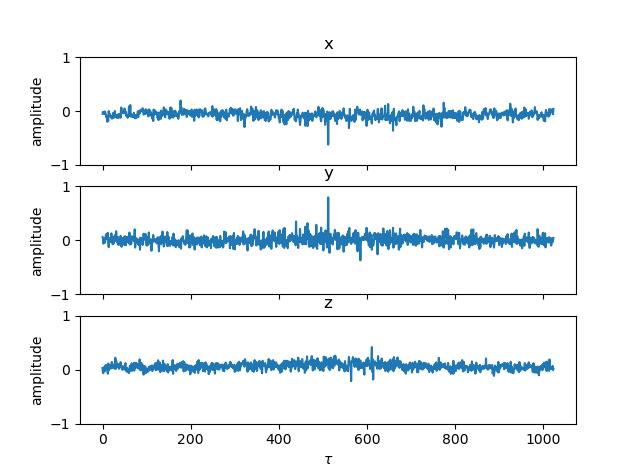
\includegraphics[width=0.7\linewidth]{Images/chap6/tdvvPlot.png}
    \captionof{figure}[Plot of a TDVV for one frame]{Plot of a TDVV for one frame of a training example, decomposed into the $x$-, $y$- and $z$- dimensions.}
    \label{fig:tdvvPlot}
    \end{center}
\end{figure}

\subsection{Speaker localization as a classification problem}
\label{ss:speakerLocalizationClassification}

\begin{figure}[t]
    \begin{center}
    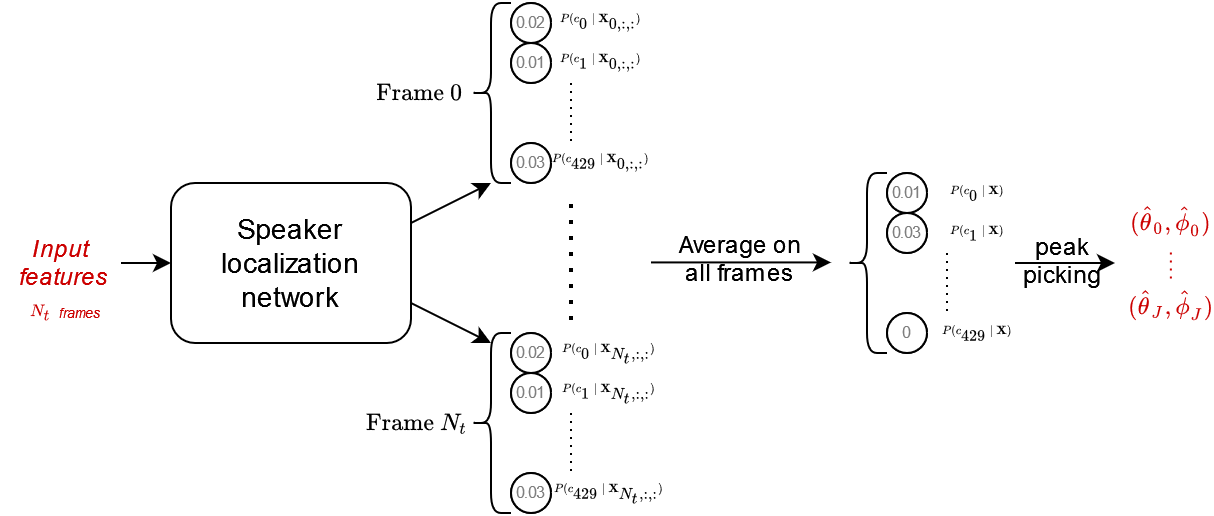
\includegraphics[width=0.8\linewidth]{Images/chap6/multiLocalizationClassification.png}
    \captionof{figure}[Speaker localization as a classification problem]{Illustration of a speaker localization system addressed as a classification problem.}
    \label{fig:multiLocalizationClassification}
    \end{center}
\end{figure}

As for speaker counting, we consider speaker localization as a classification problem, similarly to \cite{perotin_crnn-based_2018}. Fig.~\ref{fig:multiLocalizationClassification} illustrates the general classification approach we take for speaker localization, with an arbitrary NoS. From the microphone array point of view, and with the microphone array center taken as the origin of a spherical coordinate system, the DoA space is represented as a unit sphere. This 2D sphere is discretized into several regions, which will act as the classes, with the following discrete values for the source azimuth $\theta \in [-180^{\circ},180^{\circ}]$ and the source elevation $\phi \in [-90^{\circ},90^{\circ}]$:
\begin{equation}
    \left\{ 
    \begin{aligned} 
      \phi_p   &= -90^{\circ} + \frac{p}{P} \times 180^{\circ} \text{, for } p \in \{0, ..., P\} \\
      \theta_q^p &= -180^{\circ} + \frac{q}{Q_p+1} \times 360^{\circ}  \text{, for } q \in \{0, ..., Q_p\}
    \end{aligned}
    \right. ,
\end{equation}
where $P = \lfloor \frac{180}{\alpha} \rfloor$, $Q_p = \lfloor \frac{360}{\alpha} cos \phi_p \rfloor$ and $\alpha$ is the grid resolution in degrees \footnote{Note that we also used the notation $p$ to design the acoustic pressure and $Q$ for the number of Ambisonics channels, however we believe that it does not lead to confusion.}. In all our experiments, we set $\alpha = 10$\textdegree, so that we end up with $429$ DoA regions, each one represented as a class $c_i, i \in \{1,...,429\}$ for the network.

The neural network is trained to estimate a probability $P(\theta_q^p, \phi_p \mid \mathbf{X}_{t,:,:})$ that a sound source is present in region $(\theta_q^p, \phi_p)$, for each region, and for each frame from an input feature $\mathbf{X}$. We then average the probability distributions over all frames in the input sequence to obtain one final distribution $P(\theta_q^p, \phi_p \mid \mathbf{X})$. As we consider the single-source scheme in this chapter, the peak-picking stage simplifies as extracting the direction with the highest probability to be the estimated DoA:
\begin{equation}
    (\hat{\theta},\hat{\phi}) = \argmax_{(\theta_q^p,\phi_p)_{p \in [0,P],q\in[0,Q_p]}} P(\theta_q^p,\phi_p \mid \mathbf{X}).
\end{equation}

\subsection{Neural network architecture}

\begin{figure}[t]
    \begin{center}
    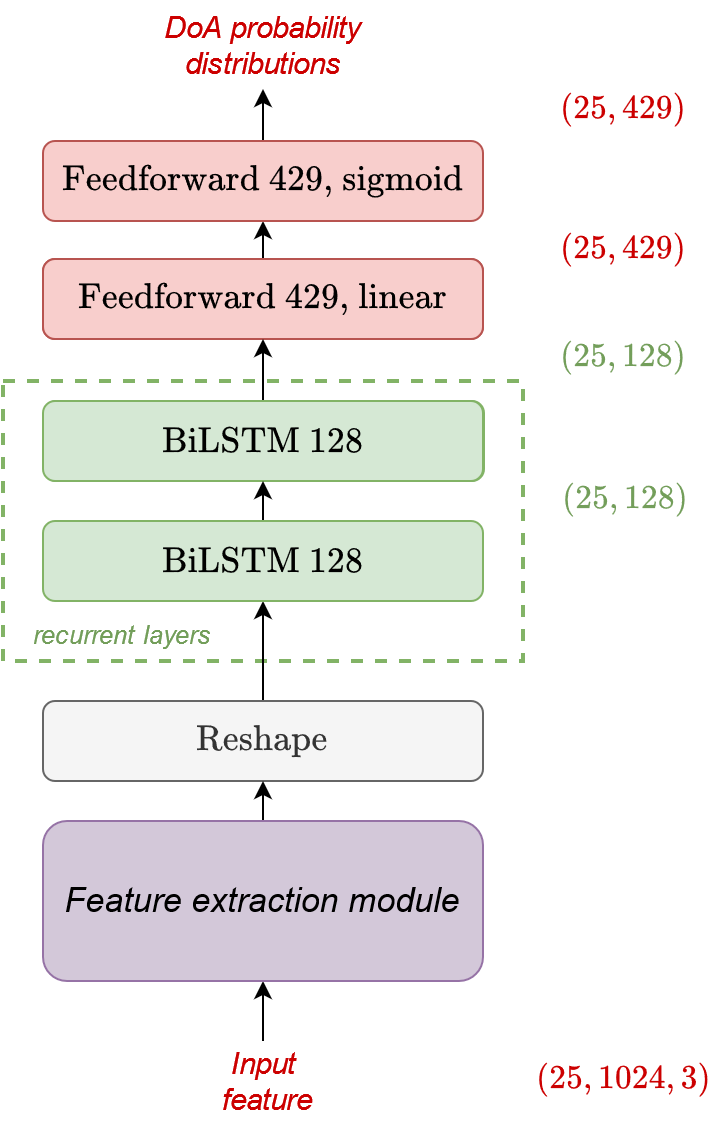
\includegraphics[width=0.5\linewidth]{Images/chap6/genericTDVVnetworkArchitecture.png}
    \captionof{figure}[General architecture of the single-speaker localization neural network]{General architecture of the neural network used for single-speaker localization. The input feature is fed into a feature extraction module whose components change according to the experiment. A recurrent module with 2 bidirectional LSTM layers is then used in a sequence-to-sequence manner, and the LSTM output vector corresponding to each frame is fed into a block of two fully-connected layers, the last one acting as the output layer. At the end, we end up with a probability distribution over the discretized DoA space for each input frame.}
    \label{fig:genericTDVVnetworkArchitecture}
    \end{center}
\end{figure}

Many neural network architectures are explored to improve the single-source localization accuracy. An illustration of a generic architecture can be found in Fig.~\ref{fig:genericTDVVnetworkArchitecture}. The input feature $\mathbf{X}$ presented above is fed into the input layer of the neural network. After a feature extraction module which will change according to the experiment, a recurrent module made of two bidirectional LSTM layers is used. These LSTM layers are used in a sequence-to-sequence manner so that each input frame leads to a new vector. In these layers, we use the same activation functions as described in Section~\ref{ss:lstm}. Then, each output vector of the second LSTM layer goes into a first feedforward layer with $128$ units and linear activation. Finally, another feedforward layer is used as the output layer, with $429$ units (one for each DoA region) and a sigmoid activation function. The use of dropout justifies the idea of using two feedforward layers with the first one using a linear activation.


%-----------------------------------------------
%  EXPERIMENTAL PROTOCOL
%-----------------------------------------------
\section{Experimental protocol}

\subsection{Audio parameters}

We use the same audio parameters as in Chapter~\ref{chap:counting}. The audio signals are sampled at $16$~kHz. Both STFT and inverse STFT are computed with a Tukey window ($\alpha = 0.5$) of length $1\,024$ samples and an overlap of $50$\%. The motivation for this choice of the window function is to reduce the signal distortion within the frame, so that the derived TDVV features remain accurate.

\subsection{Training parameters}

The neural networks are trained using the binary cross-entropy as the loss function and the Adam optimizer with a starting learning rate of $10^{-3}$, $\beta_1 = 0.9$, $\beta_2=0.999$, and $\epsilon = 10^{-7}$. During training, a dropout layer is used between the feedforward layers, with a dropout rate of $0.3$. We also monitor the network accuracy on the validation dataset during the training phase. If the accuracy does not improve for $10$ epochs, the learning rate is reduced by a factor $2$, and if it does not improve for $20$ epochs, we stop the training and keep the best performing model. The maximum number of epochs is set to $300$.

\subsection{Training data}
\label{ss:tdvvTrainingData}

The training dataset is generated in a similar way as for the speaker counting network, presented in \ref{ss:countingTrainingData}, except that we do not aim to generate conversation-like mixtures. We instead create $1$-s mixtures with a continuous speech coming from a static source.

We first generate a set a SRIRs with the image-source method \cite{allen_image_1979} using an adaptation of the RIR generator \cite{habets_room_2006} to the Ambisonics format. The SRIRs are generated with the following protocol. In order be sure that every class is well represented, \emph{i.e.}, every DoA is present with the same amount in the training phase, we first select a random DoA. Then, we pick random room dimensions in the range $[2,10]$~m, $[2,10]$~m and $[2,3]$~m, for the width, length, and height, respectively, as well as the reverberation time RT60 between $200$ and $800$~ms. Next, the microphone array is randomly positioned somewhere in the room so that it is at least at $0.5$~m from the walls. The first source position is randomly picked at a distance between $1$ and $3$~m from the microphone array with respect to the DoA selected at the beginning of the procedure. If such a constraint is not applicable (\emph{i.e.}, it forces the first source to be outside of the room), we restart the algorithm with new room dimensions. We generate a total of $128\,700$ SRIRs.

To generate the speech signals, we use the TIMIT corpus \cite{garofolo_timit_1993}, as in Chapter~\ref{chap:counting}. For each generated SRIR, we extract speech excerpts containing $1$~s of continuous speech, which we convolve with the SRIR to create a reverberant speech signal. A diffuse noise is added to the convolved speech signal with a random SNR between $0$ and $20$~dB. The diffuse noise is created by first picking a random noise signal in the same noise dataset as in Chapter~\ref{chap:counting}, and convolving it with the average of the diffuse parts of two random measured SRIRs.

The validation dataset is generated in the exact same way, based on $1\,287$ SRIRs. We took care of using different speech and noise signals, as well as new random seeds to unmatch from the random pick used in the generation of the training dataset.

The overall process results in a total of around $35$~hours of training data and $22$~minutes of validation data.

\subsection{Testing data}
\label{ss:tdvvTestData}

To evaluate our neural networks, we use two testing datasets, one with simulated SRIRs and another with recorded SRIRs. 

The first one is created using the same procedure as the training and validation sets. As we did for validation data, we take care of using new seeds for random picking, new speech signals and new noise signals to generate the testing data. We thus create a total of $22$~minutes of testing data with simulated SRIRs. The speech signals in the second dataset are created in the same way as the first one, but using real SRIRs recorded with an EigenMike in a real reverberant room. The room is $4$~m long, $7$~m wide and $2.5$~m high, and the RT60 is around $500$~ms. The microphone array are placed in $36$ positions, and for each one $16$ loudspeakers emitted a sweep signal to gather a total of $576$ SRIRs.

\subsection{Baseline}

\begin{figure}[t]
    \begin{center}
    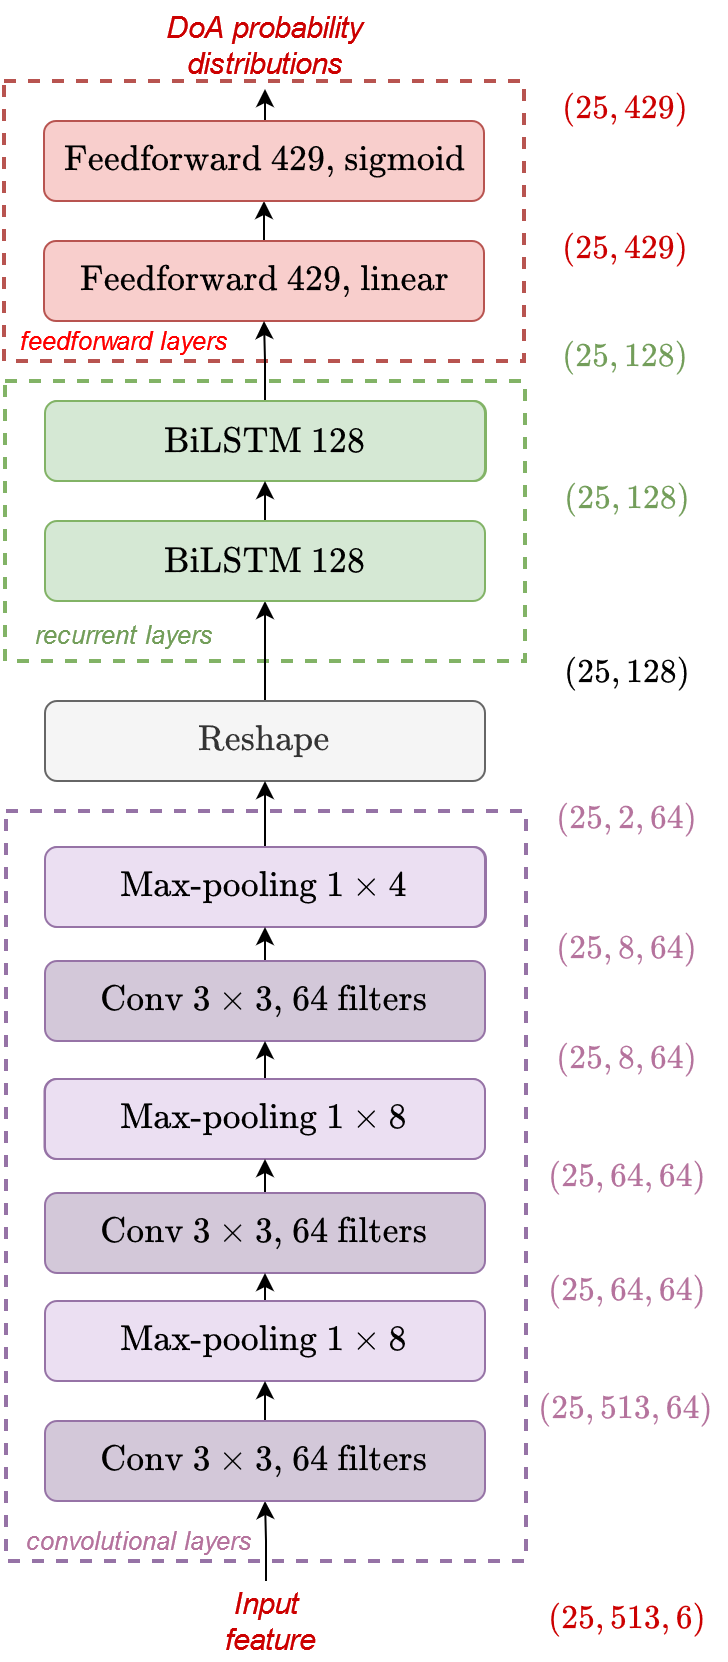
\includegraphics[width=0.4\linewidth]{Images/chap6/perotinCRNN.png}
    \captionof{figure}[Baseline localization CRNN adopted in \cite{perotin_crnn-based_2019}]{Baseline localization CRNN adopted in \cite{perotin_crnn-based_2019}.}
    \label{fig:perotinCRNN}
    \end{center}
\end{figure}

As a baseline, we use the CRNN proposed by Perotin \emph{et al.} in \cite{perotin_crnn-based_2018}, from which we draw inspiration when designing several networks during the experiments. The baseline architecture is illustrated in Fig.~\ref{fig:perotinCRNN}. The main difference with our approach is that the input feature was composed of the real and imaginary parts of the FO-PIV (see Section~\ref{ss:pseudointensityVector}). The feature extraction module is composed of $3$ convolutional layers, with $64$ convolution kernels of size $3 \times 3$, and each one is followed by a max-pooling layer with pooling sizes $1 \times 8$, $1 \times 8$ and $1 \times 4$, respectively. Dropout layers are used after each max-pooling layer during the training phase.

\subsection{Evaluation metrics}

We use two metrics to evaluate the localization performance. First, we compute the mean and median angular error (which is the angular distance between the estimated DoA and the ground-truth DoA) on the whole test dataset. On a sphere, the angular distance is defined on the unit sphere between two points $(\theta_1,\phi_1)$ and $(\theta_2,\phi_2)$ by:
\begin{equation}
    \delta((\theta_1,\phi_1),(\theta_2,\phi_2)) = \arccos \big( \sin \phi_1 \sin \phi_2 + \cos \phi_1 \cos \phi_2 \cos(\theta_1-\theta_2) \big).
\end{equation}

We also measure the classification accuracy on the test set, which is the percentage of test examples with an angular error below a certain tolerance threshold. Considering that the minimum angle between two points in the grid defined in Section~\ref{ss:speakerLocalizationClassification} is $7$\textdegree, we evaluate the classification accuracy for a tolerance threshold of $10$\textdegree~and $15$\textdegree.

%-----------------------------------------------
%  EXPERIMENTS
%-----------------------------------------------
\section{Experiments}
\label{ss:tdvvExperiments}

\subsection{TDVV against FO-PIV}

\begin{table}[t]
\centering
\subfloat[Simulated SRIRs]{
    \begin{tabular}{|c|cc|cc|}
    \hline
    \multirow{2}{*}{\textbf{Input features}} & \multicolumn{2}{c|}{\textbf{Accuracy (\%)}} & \multicolumn{2}{c|}{\textbf{Angular error (°)}} \\
    & \textbf{\textless 10°}        & \textbf{\textless 15°}        & \textbf{Mean}                  & \textbf{Median}                  \\ \hline 
    \textbf{FO-PIV}              & \textbf{95.3}                 & \textbf{99.2}                 & \textbf{5.0}                   & \textbf{4.5}                    \\
    \textbf{TDVV}                            & 77.2                 & 90.9                 & 8.1                   & 6.3                     \\ \hline
    \end{tabular}}
    
\subfloat[Real SRIRs]{
    \begin{tabular}{|c|cc|cc|}
    \hline
    \multirow{2}{*}{\textbf{Input features}} & \multicolumn{2}{c|}{\textbf{Accuracy (\%)}} & \multicolumn{2}{c|}{\textbf{Angular error (°)}} \\
    & \textbf{\textless 10°}        & \textbf{\textless 15°}        & \textbf{Mean}                  & \textbf{Median}                  \\ \hline 
    \textbf{FO-PIV}              & \textbf{67.1}                 & \textbf{83.9}                & \textbf{11.5}                   & \textbf{7.3}                     \\
    \textbf{TDVV}                            & 53.9                 & 71.2                 & 16.3                   & 9.1                     \\ \hline
    \end{tabular}}
\captionof{table}[Accuracy and angular errors of the TDVV CRNN and the baseline on the testing datasets]{Results of the localization of a single speech source with the baseline CRNN, for the FO-PIV vector and the TDVV as input feature. Best results are shown in bold.}
\label{tab:intensityVStdvv}
\end{table}


\subsubsection{Experiment objective}

The first experiment we conduct is a direct comparison of the use of the TDVV and FO-PIV as input features of the same neural network. For a fair comparison, we train the baseline CRNN, one with the TDVV and with the FO-PIV as input feature. We use the exact same training, validation and test datasets, as well as the training parameters, so that only the input features differ between the two systems.

\subsubsection{Results}

The classification accuracy and the mean and median angular errors on the two test datasets (with simulated SRIRs and real SRIRs) are shown in Table~\ref{tab:intensityVStdvv}. The angular error statistics are illustrated with boxplots and violin plots in Fig.~\ref{fig:boxplots_intensityVStdvv}.

\begin{figure}[t]
    \begin{center}
    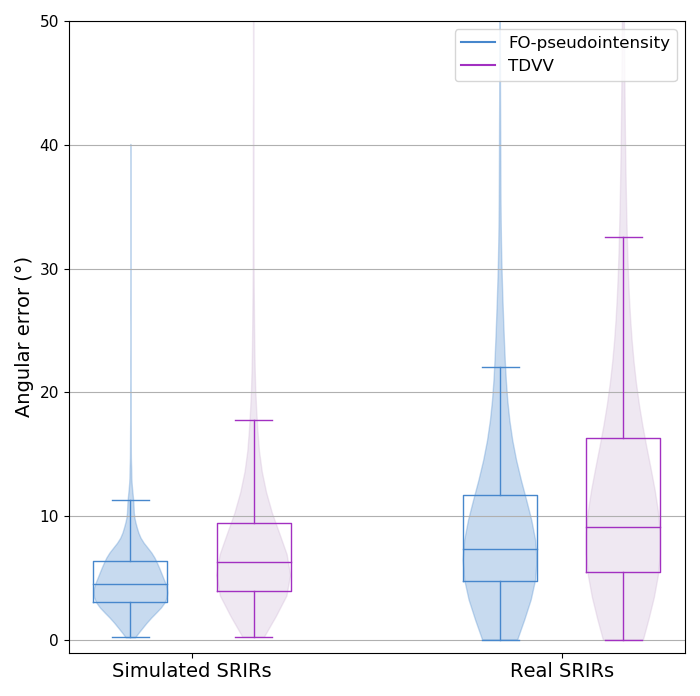
\includegraphics[width=0.5\linewidth]{Images/chap6/boxplots_intensityVStdvv.png}
    \captionof{figure}[Boxplots of the angular errors of the CRNN with TDVV and the baseline evaluated on the testing datasets]{Distribution statistics on the angular error of the CRNN with TDVV and the baseline on both testing datasets. Boxplots show the first and third quartiles as well as the median value. Superposed to each boxplot is shown the corresponding violin plot, which is an estimation of the probability density function of the statistical distribution.}
    \label{fig:boxplots_intensityVStdvv}
    \end{center}
\end{figure}

On the dataset created with simulated SRIRs, we see that the CRNN using the TDVV as input underperforms the baseline, with a notable decrease in performance. The baseline proves to be very accurate for single-source localization \cite{perotin_crnn-based_2018} with $99.2$\% accuracy with an angular tolerance of $15$\textdegree and $95$\% accuracy for a tolerance of $10$\textdegree. The CRNN using the TDVV as input only achieves $90.9$\% and $77.2$\% in these metrics, respectively. We also see on the boxplots and violin plots that the angular errors for the TDVV are more scattered than for the FO-PIV.

Regarding the dataset with real SRIRs, the observations are similar, with a drop in accuracy by around $13$\% for the TDVV in comparison to the FO-PIV, for both  $10$\textdegree~and $15$\textdegree tolerances. By using the TDVV as input feature, we increase the mean angular error by almost $5$\textdegree. The violin plots suggest that both CRNNs provide less consistent results on data generated with the real SRIRs, compared to the data generated with the simulated SRIRs.

All these results show that replacing the FO-PIV with the TDVV as neural network input feature leads to a notable decrease in localization performance. Whereas this new representation was shown to be meaningful on a theoretical point of view, it seems that the CRNN has more difficulties to extract the relevant information for DoA estimation than with the FO-PIV. This motivates us to conduct further experiments to improve the architecture, in order to give the neural network more capability to extract more relevant features.

\subsection{CRNN with dilated convolutions}

\subsubsection{Experiment objective}

\begin{figure}[t]
    \centering
    \subfloat[Feature extraction module with dilated convolutions]{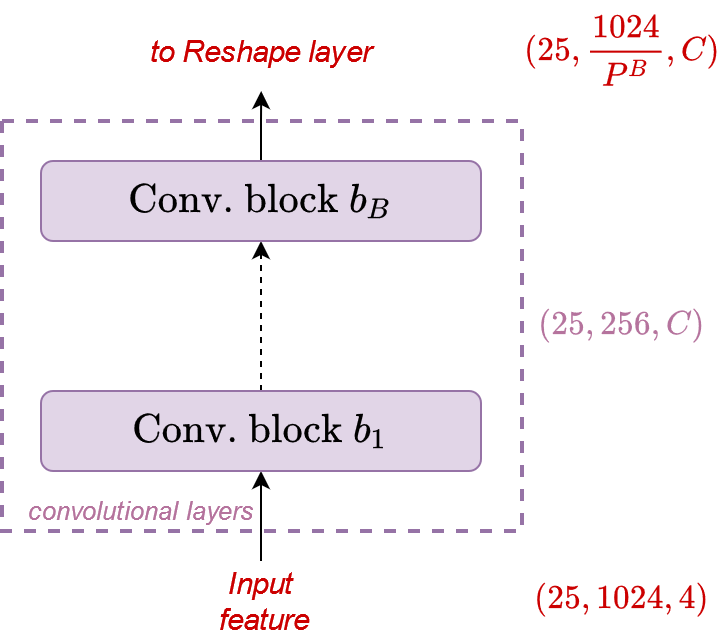
\includegraphics[width=0.40\linewidth]{Images/chap6/dilatedFeatureExtractionModule.png}\label{fig:TDVVdilatedArchitecture}}
    \hspace{1cm}
    \subfloat[Convolutional block with dilated convolution kernels]{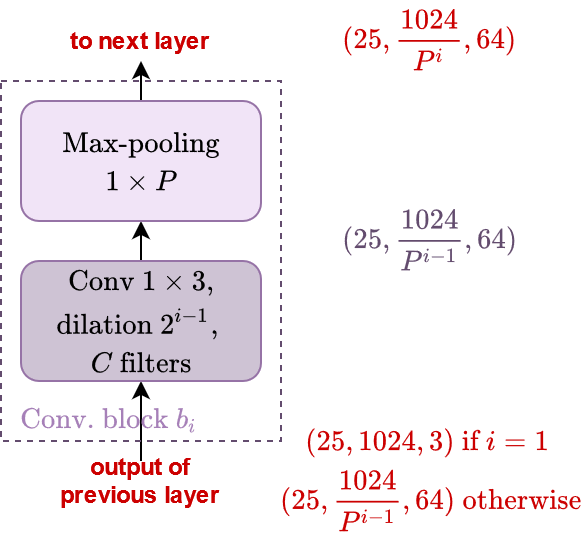
\includegraphics[width=0.40\linewidth]{Images/chap6/TDVVConvBlock.png}\label{fig:TDVVdilatedConvBlock}}
    
    \captionof{figure}[Feature extraction module with dilated convolutional layers]{Feature extraction module with $B$ convolutional blocks consisting of a convolutional layer with increasing dilation factor followed by a max-pooling layer.}
    \label{fig:TDVVdilatedConv}
\end{figure}

The previous experiment showed us that the CRNN from \cite{perotin_crnn-based_2018} makes better use of the FO-PIV than the TDVV as input feature. One reason might be because the baseline architecture has been tuned for the use of FO-PIV and thus is not suitable for feature extraction from the TDVV. We then might need a more adapted neural network for this new representation. Recalling the theoretical derivation of the TDVV in Section~\ref{ss:tdvv}, we see that it contains information about certain reflections at some specific delay $\tau$. One idea is then to give the network more flexibility during the feature extraction stage in order to process the relevant reflection components, indexed by several $\tau$ which are sometimes far from each other in the TDVV.

Dilated convolutions seem to be good candidates for that purpose because they can process data points which are not contained in a neighbouring area, without taking the in-between points into account. For this reason, we decide to replace the classical $3 \times 3$ convolution kernels with dilated kernels of size $1 \times 3$ so that the process is done only along the TDVV delay axis, separately for each frame. In that way, the TDVV information is not mixed across the frames in the convolutional layers, the temporal analysis being reserved for the subsequent layers. Fig.~\ref{fig:TDVVdilatedArchitecture} shows an illustration of the network architecture we adopt. We replace all the convolution layers from the baseline architecture with a series of $B$ dilated convolution blocks illustrated in Fig.~\ref{fig:TDVVdilatedConvBlock} where $B$ is an hyperparameter in our experiments. These blocks are made of one convolutional layer with $C$ convolution kernels of size $1 \times 3$ and a dilation factor which doubles at each additional block, starting with $l=1$, and then followed by a max-pooling layer of size $1 \times P$. The idea behind this increasing dilation factor is borrowed from the WaveNet architecture \cite{oord_wavenet:_2016}, whose authors showed that it increases the receptive field of the convolutional layer. In our case the receptive field spans the $\tau$ axis.


We train this neural network for several hyperparameter values. We stack up from $B=2$ (thus with dilation factors $l=1,2$) to $B=4$ ($l=1,2,4,8$) convolutional blocks with $C=32$ kernels and pooling sizes $P=0,2,4$ (when $P=0$ we do not use any max-pooling layers at all). For $P=4$ (which gives the most conclusive results as we will see below), we also try using $C=64$ kernels. Table~\ref{tab:TDVVdilatedNetworksParameters} summarizes the different tested configurations with the resulting number of parameters constituting the neural networks, along with the baseline for comparison.


\begin{table}[t]
\centering
\begin{tabular}{|c|ccc|c|}
\hline
\textbf{Model label}   & \textbf{$B$}                & \textbf{$P$}                & \textbf{$C$} & \textbf{\# parameters}             \\ \hline
Baseline      &   /                 &    /                &  /   & 578\,927                  \\ \hline
Dil-B2-P0-C32* & \multirow{4}{*}{4}                  & 0                  & 32  & 17\,155\,951              \\
Dil-B2-P2-C32 &                    & 2                  & 32  & 2\,475\,887               \\
Dil-B2-P4-C32 &                    & 4 & 32  & 640\,879                  \\
Dil-B2-P4-C64 &                    & 4                   & 64  & 921\,839                  \\ \hline
Dil-B3-P0-C32* & \multirow{4}{*}{3} & 0                  & 32  & 17\,159\,155              \\
Dil-B3-P2-C32* &                    & 2                  & 32  & 1\,430\,515               \\
Dil-B3-P4-C32 &                    & 4 & 32  & 447\,475                  \\
Dil-B3-P4-C64 &                    & 4                   & 64  & 541\,075                  \\ \hline
Dil-B4-P0-C32* & \multirow{4}{*}{4} & 0                  & 32  & 17\,162\,259              \\
Dil-B4-P2-C32* &                    & 2                  & 32  & 1\,433\,619 \\
Dil-B4-P4-C32 &                    & 4 & 32  & 450\,579                  \\
Dil-B4-P4-C64 &                    & 4                   & 64  & 553\,427\\    
\hline
\end{tabular}
\captionof{table}[Hyperparameter configurations of the dilated CRNN and number of parameters]{Summary of all tested configurations of hyperparameter values with the resulting number of parameters constituting the neural network. Note that the baseline number of parameters is also given whereas it is not based on dilated convolutional blocks. Model labels marked with an asterisk are those which do not manage to train properly, resulting in random predictions.}
\label{tab:TDVVdilatedNetworksParameters}
\end{table}

\subsubsection{Results}

For reasons that are not yet well identified, several sets of hyperparameters lead to an erratic network training (even after we retrain them again to make sure it is not a bug). Fig.~\ref{fig:erraticTraining} shows the validation accuracy evolution during such a training, as an example for model \textit{Dil-B2-P0-C32}. Models that we are not able to train properly are indicated with an asterisk after their label in Table~\ref{tab:TDVVdilatedNetworksParameters}. Looking at the number of parameters of these wrongly trained model, there seems to be a correlation between a high number of parameters and an erratic training. As these models do not employ a lot of pooling in the convolutional blocks, the second tensor dimension at the output of the reshape layer is quite large, implying that most of the network parameters are used to map this dimension to the BiLSTM dimension of size $64$. For example, for $B=2$, $C=32$, and no pooling, the shape at the output of the reshape layer is $(T,32\,768)$, resulting in $16\,810\,496$ parameters only for the first BiLSTM layer. This high number of parameters at one specific layer of the network could be the reason why it is hard to train. However, this problem happens also for relatively small models such as \textit{Dil-B3-P2-C32} and \textit{Dil-B4-P2-C32} (about $1.5$~M parameters); we still miss a fully satisfying explanation of this issue.

\begin{figure}[t]
    \begin{center}
    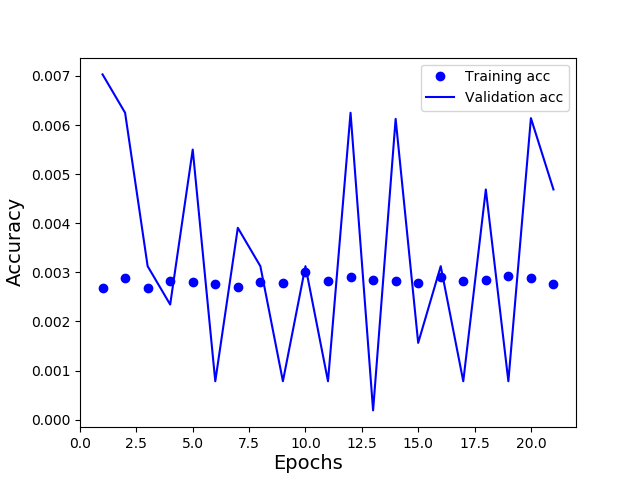
\includegraphics[width=0.4\linewidth]{Images/chap6/erraticTraining.png}
    \captionof{figure}[Training and validation accuracy evolution of an erratic training]{Training and validation accuracy evolution of the erratic training of model Dil-B2-P0-C32. We clearly see that the network does not learn, which leads to non-increasing accuracy on the validation set. Note that the accuracy is bounded by $100$\%.}
    \label{fig:erraticTraining}
    \end{center}
\end{figure}

Due to these still open problems, we present only the results for a portion of our experiments. We do not consider all the experiments leading to a functional network training. Instead, we limit the results to a subset of all configurations which allows us to rigorously compare several hyperparameter values. Therefore, since the pooling size seems to be important for a successful training, we evaluate only the models with $P=4$, which allows us to compare the different numbers of convolutional blocks and kernels.

\begin{table}[t]
\centering
\subfloat[Simulated SRIRs]{
    \begin{tabular}{|c|cc|cc|}
    \hline
    \multirow{2}{*}{\textbf{Model label}} & \multicolumn{2}{c|}{\textbf{Accuracy (\%)}}     & \multicolumn{2}{c|}{\textbf{Angular error (°)}} \\
                                          & \textbf{\textless 10°} & \textbf{\textless 15°} & \textbf{Mean}         & \textbf{Median}         \\ \hline
    Baseline CRNN with FO-PIV                   & \textbf{95.3}          & \textbf{99.2}          & \textbf{5.0}          & \textbf{4.5}            \\ 
    Baseline CRNN with TDVV                    & 77.2          & 90.9          & 8.1          & 6.3            \\ \hline
    Dil-B2-P4-C32                & 58.4                   & 75.4                   & 15.4                  & 8.6                     \\
    Dil-B2-P4-C64                & 69.3                    & 85.2                    & 10.3                  & 7.3                     \\
    Dil-B3-P4-C32                & 47.9                   & 70.5                   & 19.8                  & 10.3                    \\
    Dil-B3-P4-C64                & 70.9                   & 87.1                   & 9.6                   & 7.1                     \\
    Dil-B4-P4-C32                & 61.8                   & 79.3                   & 16.1                  & 8.2                     \\
    Dil-B4-P4-C64                & 68.1                   & 85.5                   & 10.5                  & 7.3                     \\ \hline
    \end{tabular}}
    
\subfloat[Real SRIRs]{
    \begin{tabular}{|c|cc|cc|}
    \hline
    \multirow{2}{*}{\textbf{Model label}} & \multicolumn{2}{c|}{\textbf{Accuracy (\%)}}     & \multicolumn{2}{c|}{\textbf{Angular error (°)}} \\
                                          & \textbf{\textless 10°} & \textbf{\textless 15°} & \textbf{Mean}         & \textbf{Median}         \\ \hline
    Baseline                     & \textbf{67.1}          & \textbf{83.9}          & \textbf{11.5}         & \textbf{7.34}           \\ \hline
    Dil-B2-P4-C32                & 42.4                   & 61.4                   & 26.8                  & 11.9                    \\
    Dil-B2-P4-C64                & 50.7                   & 68.1                   & 21.8                  & 9.8                     \\
    Dil-B3-P4-C32                & 35.8                   & 55.7                   & 35.2                  & 13.2                    \\
    Dil-B3-P4-C64                & 49.1                   & 67.4                   & 18.4                  & 10.1                    \\
    Dil-B4-P4-C32                & 47.0                   & 62.9                   & 28.6                  & 10.7                    \\
    Dil-B4-P4-C64                & 52.0                   & 70.3                   & 21.2                  & 9.6                     \\ \hline
    \end{tabular}}

\captionof{table}[Accuracy and angular errors of the dilated CRNNs with TDVV and the baseline on the testing datasets]{Accuracy and angular errors of the dilated CRNNs with TDVV and the baseline on the testing datasets. Best results are in bold.}
\label{tab:TDVV_dilatedConv}
\end{table}

\begin{figure}[ht]
    \begin{center}
    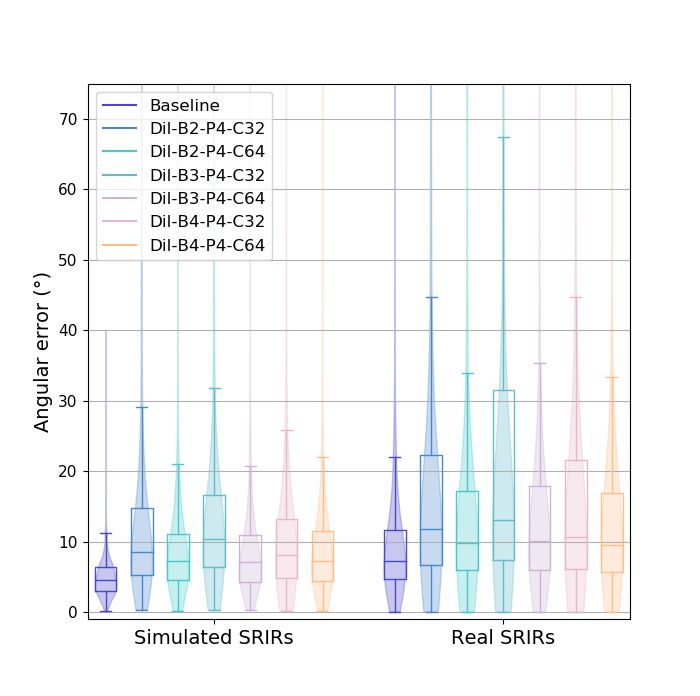
\includegraphics[width=0.5\linewidth]{Images/chap6/boxplots_dilatedConv.png}
    \captionof{figure}[Boxplots of the angular errors of the dilated CRNNs with TDVV and the baseline evaluated on the testing datasets]{Distribution statistics on the angular error of the dilated CRNNs with TDVV and the baseline on both testing datasets.}
    \label{fig:boxplots_dilatedConv}
    \end{center}
\end{figure}

As we can see in Table~\ref{tab:TDVV_dilatedConv} and Fig.~\ref{fig:boxplots_dilatedConv}, the performance of the dilated CRNNs is still far from the baseline. We even lose in performance compared to the baseline architecture with the TDVV as input feature (see Table~\ref{tab:intensityVStdvv}). Using simulated SRIRs, the localization accuracy for this architecture was $90.9$\% for a tolerance of $15$\textdegree, while it drops between $70.5$ and $87.7$\% .when considering the best-performing dilated CRNN. With real SRIRs, the accuracy decrease is 



a bit less pronounced, going from $71.2$\% with the baseline architecture to between $55.7$\% and $70.3$\%.

When comparing the dilated CRNNs with each other, we see that using $C=64$ convolution kernels instead of $C=32$ leads to better results in all cases. For instance with real SRIRs, the mean angular error goes from $26.8$\textdegree~to $21.8$\textdegree~when $B=2$, or from $35.2$\textdegree~to $21.2$\textdegree~when $B=4$. Moreover, there is a tendency that the performance increases when $B$ increases, \emph{i.e.}, using more convolutional blocks results in a more accurate network.

It is not clear why we observe a drop in performance with this new feature extraction module. In the baseline architecture, only $3$ convolutional layers with $64$ kernels are used, and the pooling size is larger. In our proposal, even with $C=64$ and $P=4$, we witness a decrease in accuracy. One important change we made is the replacement $3 \times 3$ max-pooling block by $1 \times 3$ pooling, which could be the cause of this decline, although it seems surprising to be the only explanation. It could be instructive to evaluate these models with $3 \times 3$ max-pooling to assess this idea, however we did not have time to do it.

To conclude this experiment, the proposed feature extraction module does not allow to improve over the baseline performance. It even further deteriorates compared to using the baseline architecture with the TDVV as input feature. However, we learn that using a relatively large max-pooling is necessary to avoid having too many parameters and an untrainable network, and that using $C=64$ kernels in the majority of convolutional blocks leads to better results.

\subsection{CRNN with dilated convolutions and residual connections}
\subsubsection{Experiment objective}

In order to improve the feature extraction module, we try adding residual connections to the CRNN to help stabilising the training of a network. The idea is that each feature map is reused in the next layers, to hopefully allow the network more flexibility in producing an informative representation for the localization task. We use a similar architecture as before, with the difference that each convolutional block contains two convolutional layers with a residual connection, as illustrated in Fig.~\ref{fig:TDVVResidualConvBlock}. As we can see, the output of the first convolutional layer is concatenated with the output of the second one, leading to a total of $2C$ feature maps. Again, the second dimension of the resulting tensor is reduced using a max-pooling layer. We experimente with different numbers of such blocks ($B=1,2,3,4,5$). This results in more convolutional layers ($10$ when $B=5$), therefore, we modify the dilation factor progression with all successive integer values; that is, in the first block we have $l=1$ for the first convolutional layer and $l=2$ for the second one, then for the second block we have $l=3$ and $l=4$, and so forth. We set the remaining hyperparameter values to the values that produces the best results in the previous experiment ($C=64$, $P=4$). Table~\ref{tab:TDVVresidualNetworksParameters} sums up the tested configurations.

\begin{figure}[ht]
    \begin{center}
    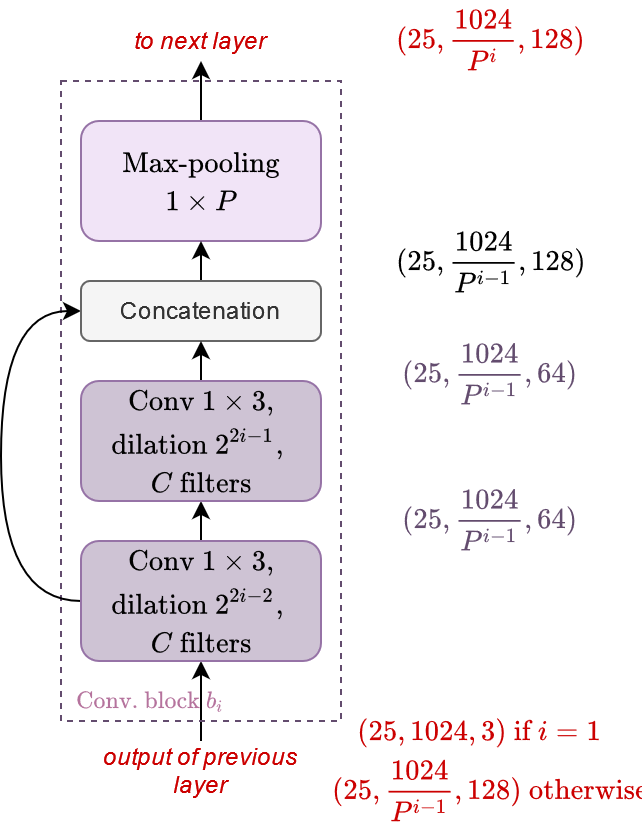
\includegraphics[width=0.5\linewidth]{Images/chap6/TDVVResidualConvBlock.png}
    \captionof{figure}[Convolutional block with a residual connection]{Convolutional block with two convolutional layers and with a residual connection propagating the output of the first block to the output of the second one. They are both concatenated before fed into a max-pooling layer.}
    \label{fig:TDVVResidualConvBlock}
    \end{center}
\end{figure}

\begin{table}[ht]
\centering
\begin{tabular}{|c|ccc|c|}
\hline
\textbf{Model label}   & \textbf{$B$} & \textbf{$P$}       & \textbf{$C$}        & \textbf{\# parameters} \\ \hline
Baseline      & /            & /                  & /                   & 578\,927               \\ \hline
Res-B1-P4-C64* & 1            & 4 & 64 & 17\,162\,315  \\
Res-B2-P4-C64* & 2            & 4 & 64 & 4\,616\,595   \\
Res-B3-P4-C64* & 3            & 4 & 64 & 1\,508\,059   \\
Res-B4-P4-C64 & 4            & 4 & 64 & 535\,043      \\
Res-B5-P4-C64 & 5            & 4 & 64 & 599\,403      \\ \hline
\end{tabular}
\captionof{table}[Hyperparameter configurations of the residual dilated CRNN and number of parameters]{Summary of all tested configurations of hyperparameter values with the resulting number of parameters constituting the residual CRNN. Model architectures marked with an asterisk are those which do not managed to train properly, resulting in random predictions.}
\label{tab:TDVVresidualNetworksParameters}
\end{table}

\subsubsection{Results}

\begin{table}[ht]
\centering
\subfloat[Simulated SRIRs]{
    \begin{tabular}{|c|cc|cc|}
    \hline
    \multirow{2}{*}{\textbf{Model label}} & \multicolumn{2}{c|}{\textbf{Accuracy (\%)}}          & \multicolumn{2}{c|}{\textbf{Angular error (°)}} \\
                                          & \textbf{\textless 10°} & \textbf{\textless 15°} & \textbf{Mean}       & \textbf{Median}       \\ \hline
    Baseline                     & \textbf{95.3}          & \textbf{99.2}          & \textbf{5.0}        & \textbf{4.5}          \\ \hline
    Res-B4-P4-C64                & 61.3                   & 80.3                   & 13.0                & 8.2                   \\
    Res-B5-P4-C64                & 26.4                   & 45.2                   & 21.1                & 16.8                  \\ \hline
    \end{tabular}}
    
\subfloat[Real SRIRs]{
    \begin{tabular}{|c|cc|cc|}
    \hline
    \multirow{2}{*}{\textbf{Model label}} & \multicolumn{2}{c|}{\textbf{Accuracy (\%)}}          & \multicolumn{2}{c|}{\textbf{Angular error (°)}} \\
                                          & \textbf{\textless 10°} & \textbf{\textless 15°} & \textbf{Mean}       & \textbf{Median}       \\ \hline
    Baseline                     & \textbf{67.1}          & \textbf{83.8}          & \textbf{11.5}       & \textbf{7.3}          \\ \hline
    Res-B4-P4-C64                & 47.5                   & 65.4                   & 23.2                & 10.3                  \\
    Res-B5-P4-C64                & 22.7                   & 40.4                   & 29.8                & 17.8                  \\ \hline
    \end{tabular}}
    
\captionof{table}[Accuracy and angular errors of the residual CRNNs with TDVV and the baseline on the testing datasets]{Accuracy and angular errors of the residual CRNNs with TDVV and the baseline on the testing datasets. Best results are in bold.}
\label{tab:TDVV_residualConv}
\end{table}

\begin{figure}[ht]
    \begin{center}
    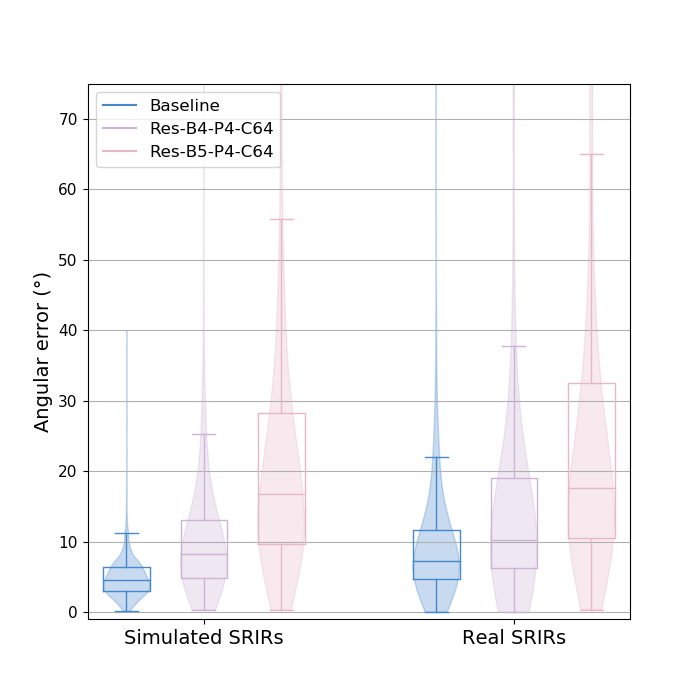
\includegraphics[width=0.5\linewidth]{Images/chap6/boxplots_residualConv.png}
    \captionof{figure}[Boxplots of the angular errors of the residual CRNNs with TDVV and the baseline evaluated on the testing datasets]{Distribution statistics on the angular error of the residual CRNNs with TDVV and the baseline on both testing datasets.}
    \label{fig:boxplots_residualConv}
    \end{center}
\end{figure}

The residual connections fail to stabilise training, since the models with too many parameters (for $B=1,2,3$) do not train properly, leading to random results. We thus present the results for $B=4,5$ in Table~\ref{tab:TDVV_residualConv} and Fig.~\ref{fig:boxplots_residualConv}.

As we can see, the results are even worst than all other experiments. While the model labelled \textit{Res-B4-P4-C64} reaches a reasonable performance slightly below the dilated CRNNs with $C=64$, the model \textit{Res-B4-P4-C64} results in poor performance, with only $45.2$\% accuracy with a tolerance of $15$\textdegree~with simulated SRIRs.

Although we keep the best hyperparameter values found in the previous experiment, we do not manage to improve the results by adding residual connections, and we even surprisingly worsen the localization performance. Compared to the previous models, we only change the design of the convolutional block by adding a second convolutional layer with a residual connection. Intuitively, such a modification should have a positive impact on localization performance, since it improves the flexibility of feature extraction. Unfortunately, we fail to explain the outcome of this experiment.

%-----------------------------------------------
%  CONCLUSION AND PERSPECTIVES
%-----------------------------------------------
\clearpage
\section{Conclusion and perspectives}

In this chapter we presented a series of experiments to assess the capabilities of combining neural networks with the TDVV. While many information including the DoA can be extracted from the theoretical TDVV, we saw that, in practice, the extraction of such a feature is very noisy, which motivated us to rely on the expressive power of neural networks. Throughout numerous experiments, of whom we only presented those giving interesting results, we attempted to improve single-source localization with the TDVV as input feature, compared to the use of the FO-PIV. Although the use of TDVV resulted in a fair localization accuracy, the baseline was never outperformed. We made a lot of efforts to redesign the network feature extraction module to be adapted to this new kind of input feature, without success.

The most interesting, yet difficult part of these experiments, is to understand why we did not manage to improve localization with these new features. Concerning the models that we were not able to train properly, we speculated that this was due to the too large number of parameters accumulated in one specific layer, resulting from the network design. However, the reason why using dilated convolutions and residual connections decreased the performance is not clear. While the inconclusiveness of several attempts could allow to avoid repeating the same mistakes, we believe that these ideas could lead to interesting future works due to the promising possibilities of using the TDVV with neural networks.

As we were not able to successfully exploit the TDVV's nature despite the effort of finding an adapted feature extraction module, the issue could lie in the TDVV estimation itself. In these experiments, we extracted the TDVV in a somehow \textit{naive} manner, by incorporating an \textit{epsilon} value to avoid dividing by zero, which had the effect of emphasizing noise in low SNR conditions. More elaborate estimation algorithms could be employed beforehand to help the network for better feature extraction. For example, as the TDVV is related to the relative transfer function, one could adapt RTF estimation algorithms such as \cite{shalvi_system_1996, cohen_relative_2004, gannot_signal_2001}. 

Furthermore, applying the self-attention mechanism across the delay dimension of TDVV, could be a viable alternative to (dilated) convolutions. This raises concerns with regards to computational complexity, hence an efficient implementation (\emph{e.g.}, \cite{katharopoulos_transformers_2020}) is a prerequisite.

While the inconclusiveness of all the presented attempts could allow to avoid repeating the same mistakes, we believe that these ideas could lead to interesting future works due to the promising possibilities of using the TDVV with neural networks. We still think that these ideas could really benefit source localization and that the effort should continue towards a robust TDVV estimation algorithm, as well as a neural network design conceived with the theoretical TDVV properties in mind. 
